\title{CS4248 Assignment 1}
\author{Heng Low Wee (U096901R)}
\date{}
\documentclass[fleqn,11pt]{article}
\usepackage[lmargin=0.5in,rmargin=0.5in,tmargin=0.5in,bmargin=0.5in]{geometry}
\usepackage[compact]{titlesec}
\usepackage{url}
\usepackage{amssymb,amsmath,amstext,amsgen,amsbsy,amsopn,amsfonts,mathabx,graphicx,graphics,overcite,theorem,tikz,anysize,multicol}
%\titlespacing{\section}{0pt}{*0}{*0}
%\titlespacing{\subsection}{0pt}{*0}{*0}
%\titlespacing{\subsubsection}{0pt}{*0}{*0}

\begin{document}
\maketitle
\begin{enumerate}
\item 
	\begin{align*}
	p(k) = \displaystyle \frac{\displaystyle {n \choose k}{N-n \choose n-k}}{\displaystyle {N \choose n}}
	\end{align*}
	
\item
\begin{align*}
P_{wb}(w|c_i) &= \frac{C(c_i, w)}{C(c_i) + T(c_i)}~\text{if}~C(c_i, w) > 0\\
P_{wb}(w|c_i) &= \frac{T(c_i)}{Z(c_i) \cdot (C(c_i) + T(c_i))}~\text{if}~C(c_i, w) = 0
\end{align*}
So, we need to know $C(c_i, w), C(c_i), T(c_i)~\&~Z(c_i)$\\
$V$ = \{John, loves, swimming, strengthens, our, body, jogging, is, fun, Mary\}\\
$|V| = 10$\\
$c_1:$\\
$C(c_1) = |c_1| = 7$\\
$T(c_1) = |\forall w \in V, w \in c_1| = 6$\\
$Z(c_1) = |\forall w \in V, w \not \in c_1| = 4$\\
$c_2:$\\
$C(c_2) = |c_2| = 6$\\
$T(c_2) = |\forall w \in V, w \in c_2| = 5$\\
$Z(c_2) = |\forall w \in V, w \not \in c_2| = 5$\\
\\
\begin{tabular}{| l | c | c | c | c |}
	\hline
	& \multicolumn{2}{|c|}{$P_{wb}(w|c_1)$} & \multicolumn{2}{|c|}{$P_{wb}(w|c_2)$} \\
	& $C(c_1, w)$ & wb-Smooth & $C(c_2, w)$ & wb-Smooth \\
	\hline
	body 			& 1 & $\frac{1}{7+6} = 0.0769$ & 0 & $\frac{5}{5 \times (6+5)} = 0.0909$\\
	\hline
	fun 			& 0 & $\frac{6}{4 \times (7 + 6)} = 0.115$ & 1 & $\frac{1}{6+5} = 0.0909$\\
	\hline
	is 				& 0 & 0.115 & 1 & 0.0909\\
	\hline
	jogging 		& 0 & 0.115 & 2 & 0.182\\
	\hline
	John 			& 1 & 0.0769 & 0 & 0.0909\\
	\hline
	loves 			& 1 & 0.0769 & 1 & 0.0909\\
	\hline
	Mary 			& 0 & 0.115 & 1 & 0.0909\\
	\hline
	our 			& 1 & 0.0769 & 0 & 0.0909\\
	\hline
	strengthens 	& 1 & 0.0769 & 0 & 0.0909\\
	\hline
	swimming 		& 2 & 0.154 & 0 & 0.0909\\
	\hline
\end{tabular}
\newpage
\item 
Minimum Edit Distance \\ \\ 
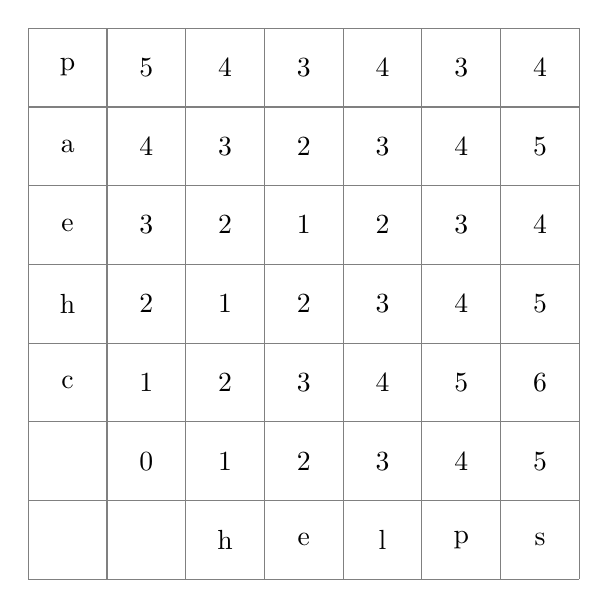
\begin{tikzpicture}
\draw[step=1cm,color=gray] (0,0) grid (7,7);
\node at (1-0.5,7-0.5) {p};
\node at (1-0.5,6-0.5) {a};
\node at (1-0.5,5-0.5) {e};
\node at (1-0.5,4-0.5) {h};
\node at (1-0.5,3-0.5) {c};

\node at (2-0.5,7-0.5) {5};
\node at (2-0.5,6-0.5) {4};
\node at (2-0.5,5-0.5) {3};
\node at (2-0.5,4-0.5) {2};
\node at (2-0.5,3-0.5) {1};
\node at (2-0.5,2-0.5) {0};

\node at (3-0.5,2-0.5) {1};
\node at (4-0.5,2-0.5) {2};
\node at (5-0.5,2-0.5) {3};
\node at (6-0.5,2-0.5) {4};
\node at (7-0.5,2-0.5) {5};

\node at (3-0.5,1-0.5) {h};
\node at (4-0.5,1-0.5) {e};
\node at (5-0.5,1-0.5) {l};
\node at (6-0.5,1-0.5) {p};
\node at (7-0.5,1-0.5) {s};

\node at (1-0.5,1-0.5) {\Huge$\bigtimes$};
\node at (2-0.5,1-0.5) {\Huge$\bigtimes$};
\node at (1-0.5,2-0.5) {\Huge$\bigtimes$};

\node at (3-0.5,3-0.5) {2};
\node at (3-0.5,4-0.5) {1};
\node at (3-0.5,5-0.5) {2};
\node at (3-0.5,6-0.5) {3};
\node at (3-0.5,7-0.5) {4};

\node at (4-0.5,3-0.5) {3};
\node at (4-0.5,4-0.5) {2};
\node at (4-0.5,5-0.5) {1};
\node at (4-0.5,6-0.5) {2};
\node at (4-0.5,7-0.5) {3};

\node at (5-0.5,3-0.5) {4};
\node at (5-0.5,4-0.5) {3};
\node at (5-0.5,5-0.5) {2};
\node at (5-0.5,6-0.5) {3};
\node at (5-0.5,7-0.5) {4};

\node at (6-0.5,3-0.5) {5};
\node at (6-0.5,4-0.5) {4};
\node at (6-0.5,5-0.5) {3};
\node at (6-0.5,6-0.5) {4};
\node at (6-0.5,7-0.5) {3};

\node at (7-0.5,3-0.5) {6};
\node at (7-0.5,4-0.5) {5};
\node at (7-0.5,5-0.5) {4};
\node at (7-0.5,6-0.5) {5};
\node at (7-0.5,7-0.5) {4};

\end{tikzpicture}
\item
Given: \\
$H(X) = \displaystyle -\sum_{x \in X} p(x) \log{p(x)}$\\
$H(X,Y) = \displaystyle -\sum_{x \in X} \sum_{y \in Y} p(x,y) \log{p(x,y)}$\\
$H(Y|X) = \displaystyle -\sum_{x \in X} \sum_{y \in Y} p(x,y) \log{p(y|x)}$\\
To verify:\\
$H(X,Y) = H(X) + H(Y|X)$
\begin{align*}
	H(X,Y) &= \displaystyle -\sum_{x \in X} \sum_{y \in Y} p(x,y) \log{p(x,y)} \\
			&= \displaystyle -\sum_{x \in X} \sum_{y \in Y} p(x,y) \log{[p(y|x)p(x)]}\\
			&= \displaystyle -\sum_{x \in X} \sum_{y \in Y} p(x,y) (\log{p(y|x)} + \log{p(x)})\\
			&= \displaystyle -\sum_{x \in X} \sum_{y \in Y} p(x,y)\log{p(y|x)} + p(x,y)\log{p(x)}\\
			&= \displaystyle -\sum_{x \in X} \sum_{y \in Y} p(x,y)\log{p(y|x)} + \left(-\sum_{x \in X} \sum_{y \in Y} p(x,y)\log{p(x)}\right)\\
			&= \displaystyle \left(-\sum_{x \in X} \sum_{y \in Y} p(x,y)\log{p(x)}\right) + \left(-\sum_{x \in X} \sum_{y \in Y} p(x,y)\log{p(y|x)}\right)\\
			&= \displaystyle \left(-\sum_{x \in X} p(x)\log{p(x)}\right) + \left(-\sum_{x \in X} \sum_{y \in Y} p(x,y)\log{p(y|x)}\right)\\
			&= H(X) + H(Y|X)
\end{align*}
\end{enumerate}

\end{document}























